\documentclass{beamer}

\usepackage[utf8]{inputenc}

\usetheme{Warsaw}

\useoutertheme{infolines}
\setbeamertemplate{blocks}[default]
\hypersetup{linkbordercolor={ 0.36 1 0.54 }}
%% \setbeamertemplate{items}[circle]

% \logo{\includegraphics[width=15px,height=15px]{/home/wulczer/flumotion.png}}

\AtBeginSubsection[]
{
  \begin{frame}{Outline}
    \tableofcontents[sectionstyle=show/shaded,subsectionstyle=show/shaded/hide]
  \end{frame}
}

\title{Replacing GEQO}
\subtitle{Join ordering via Simulated Annealing}
\author{Jan Urbanski \\ \texttt{j.urbanski@wulczer.org}}
\institute{University of Warsaw / Flumotion}
\date{\today}

\begin{document}

\frame{\titlepage}

\begin{frame}
  \tableofcontents
\end{frame}

\section{The problem}
\subsection{Determining join order for large queries}

\begin{frame}
  \frametitle{Getting the optimal join order}

  \begin{itemize}
  \item part of of planning a query is determining the order in which relations
    are joined
  \item it is not unusual to have queries that join lots of relations
  \item JOIN and subquery flattening contributes to the number or relations to
    join
  \item automatically generated queries can involve very large joins
  \end{itemize}
\end{frame}

\begin{frame}
  \frametitle{Problems with join ordering}

  \begin{itemize}
  \item finding the optimal join order is an NP-hard problem
  \item considering all possible ways to do a join can exhaust available memory
  \item not all join orders are valid, because of:
    \begin{itemize}
    \item outer joins enforcing a certain join order
    \item IN and EXISTS clauses that get converted to joins
    \end{itemize}
  \item joins with restriction clauses are preferable to Cartesian joins
  \end{itemize}
\end{frame}

\subsection{GEQO, the genetic query optimiser}

\begin{frame}
  \frametitle{Randomisation helps}

  \begin{itemize}
  \item PostgreSQL switches from exhaustive search to a randomised algorithm
    after a certain limit
  \item GEQO starts by joining the relations in any order
  \item and then proceeds to randomly change the join order
  \item genetic algorithm techniques are used to choose the cheapest join order
  \end{itemize}
\end{frame}

\begin{frame}
  \frametitle{Problems with GEQO}

  \begin{itemize}
  \item has lots of dead/experimental code
  \item there is a TODO item to remove it
  \item nobody really cares about it
  \item is an adaptation of an algorithm to solve TSP, not necessarily best
    suited to join ordering
  \item requires some cooperation from the planeer, which violates abstractions
  \end{itemize}
\end{frame}

\section{The solution}

\subsection{Simulated Annealing overview}

\begin{frame}
  \frametitle{Previous work}
  FIXME

  Twopo, the paper by the Greek, suggestions on the mailing list.
\end{frame}

\begin{frame}
  \frametitle{What is Simulated Annealing}

  \begin{columns}
    \begin{column}{7cm}
      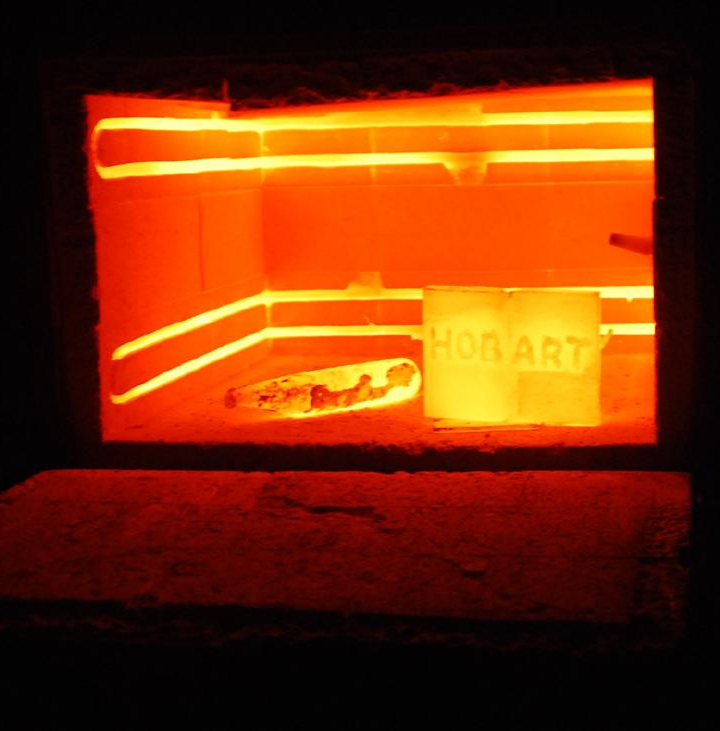
\includegraphics[width=7cm]{furnace.png}
    \end{column}
    \begin{column}{5cm}
      Annealing (...) is a process that produces conditions by heating to above
      the re-crystallization temperature and maintaining a suitable
      temperature, and then cooling.\\
      \hfill\textit{-- Wikipedia}
    \end{column}
  \end{columns}
\end{frame}

\begin{frame}
  \frametitle{The SA Algorithm cont.}

  \begin{itemize}
  \item the system starts with an initial temperature and a random state
  \item uphill moves are accepted with probability that depends on the current
    temperature
    \begin{block}{probability of accepting an uphill move}
      \begin{equation*}
        p = e^{\frac{cost_{prev} - cost_{new}}{temperature}}
      \end{equation*}
    \end{block}
  \item moves are made until equilibrium is reached
  \item temperature is gradually lowered
  \item once the system is frozen, the algorithm ends
  \end{itemize}

\end{frame}

\begin{frame}<-6>[fragile,label=sa-algorithm]
  \frametitle{The SA algorithm}

\begin{block}{Simulated Annealing}
\begin{semiverbatim}
\uncover<2->{state = \alert<7->{random\_state()}}
\uncover<6->{do \{}
\uncover<4->{    do \{}
\uncover<3->{      new\_state = \alert<8->{random\_move()}}
\uncover<3->{      if (\alert<9->{acceptable(}new\_state\alert<9->{)})}
\uncover<3->{        state = new\_state}
\uncover<4->{    \}}
\uncover<4->{    while (!\alert<10->{equilibrium()})}
\uncover<5->{    \alert<11->{reduce\_temperature()}}
\uncover<6->{\}}
\uncover<6->{while (!\alert<12->{frozen()})}
\uncover<6->{return state}
\end{semiverbatim}
\end{block}

\end{frame}

\begin{frame}<1>[label=sa-problems]
  \frametitle<1>{The SA Algorithm cont.}
  %% \frametitle<2->{SA Algorithm problems}

Implementing Simulated Annealing means solving the following problems:

  \begin{itemize}
  \item \structure<3->{finding an initial state}
  \item \alert<4->{generating subsequent states}
  \item \structure<3->{defining an acceptance function}
  \item \structure<3->{determining the equilibrium condition}
  \item \structure<3->{suitably lowering the temperature}
  \item \structure<3->{determining the freeze conditions}
  \end{itemize}

  \begin{center}
    \only<3->{Some are \structure{easy}}\only<4->{, some are \alert{hard}}
  \end{center}
\end{frame}

\againframe<6->{sa-algorithm}

\begin{frame}
  \frametitle{A visual example}
  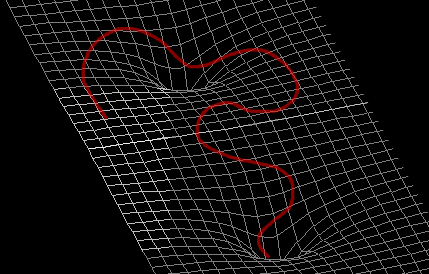
\includegraphics[width=\textwidth]{curve.png}
\end{frame}

\subsection{PostgreSQL specifics}

\begin{frame}
  \frametitle{Differences from the original algorithm}

  \begin{itemize}
  \item PostgreSQL always considers all possible paths for a relation
  \item \texttt{make\_join\_rel} is symmetrical
  \item you can have join order constraints (duh)
  \item the planner is keeping a list of all relations...
  \item ... and sometimes turns it into a hash
  \end{itemize}
\end{frame}

\begin{frame}
  \frametitle{Join order representation}

  \begin{itemize}
  \item SAIO represents joins as \alert{query trees}
  \item chosen to mimic the original algorithm more closely
  \item each state is a query tree
  \item leaves are basic relations
  \item internal nodes are joinrels
  \item the joinrel in the root of the tree is the current result
  \end{itemize}
\end{frame}

\begin{frame}<1>[label=qt-zoom]
  \frametitle<1>{Query trees}
  \framezoom<1><2>[border](1.2cm,0cm)(5.8cm,4.4cm)

  \begin{columns}
    \begin{column}{7cm}
      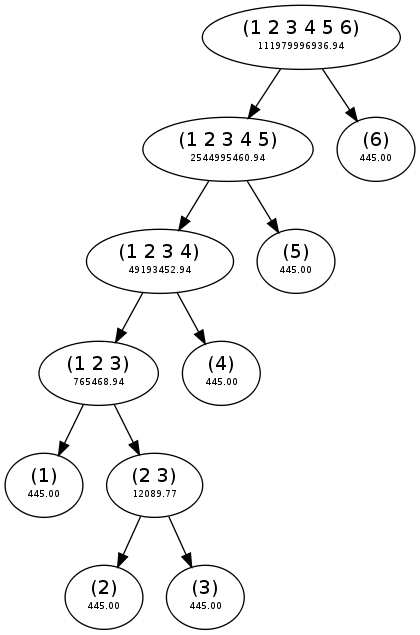
\includegraphics[width=7cm,height=8cm]{qt-example.png}
    \end{column}
    \begin{column}{5cm}
      Example query tree for a six relation join.
    \end{column}
  \end{columns}

\end{frame}

\begin{frame}
  \frametitle{Query trees cont.}

  Some useful query tree properties:

  \begin{itemize}[<+->]
  \item symmetrical (no difference between left and right child)
  \item fully determined by the tree structure and relations in leaves
  \item each node has a cost
  \end{itemize}

  \begin{center}
    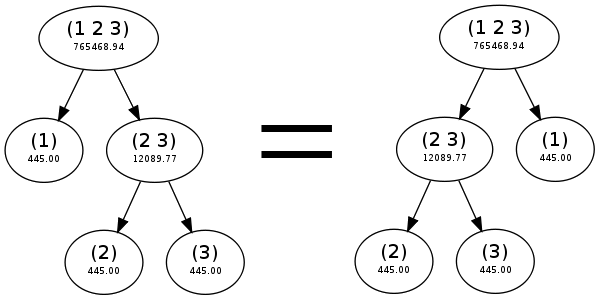
\includegraphics[width=8cm]{qt-symmetrical-1.png}<1>
    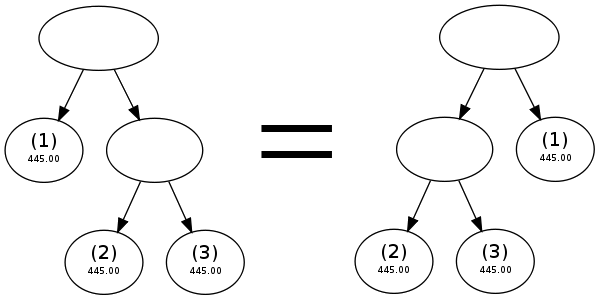
\includegraphics[width=8cm]{qt-symmetrical-2.png}<2>
    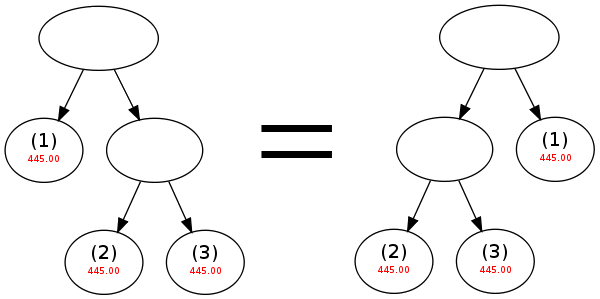
\includegraphics[width=8cm]{qt-symmetrical-3.png}<3>
  \end{center}

\end{frame}

\subsection{Query tree transformations}

\againframe<2->{sa-problems}

\begin{frame}
  \frametitle{The easy problems - initial state}

  \begin{block}{Finding an initial state}
    Make base relations into one-node trees, keep merging them on joins with
    restriction clases, forcefully merge the remaining ones using Cartesian
    joins. Results in a query tree that is as left-deep as possible.
    \\
    \hfill
    \\
    This is exactly what GEQO does.
  \end{block}
\end{frame}

\begin{frame}
  \frametitle{The easy problems - temperature}

  \begin{block}{The acceptance function}
    A uphill move is accepted with the probability that depends on the current temperature.
    $$P(accepted) = e^{\frac{cost_{prev} - cost_{new}}{temperature}}$$
  \end{block}

  \begin{block}{Lowering the temperature}
    The initial temperature depends on the number of initial relations and
    drops geometrically.
    $$initial\_temperature = I * initial\_rels$$
    $$new\_temperature = temperature * K$$ where $$0 < K < 1$$
  \end{block}
\end{frame}

\begin{frame}
  \frametitle{The easy problems - equilibrium and freezing}

  \begin{block}{Equilibrium condition}
    Equilibrium is reached after a fixed number of moves that depend on the
    number of initial relations.
    $$moves\_to\_equilibrium = N * initial\_rels$$
  \end{block}

  \begin{block}{Freezing condition}
    The system freezes if temperature falls below 1 and a fixed number of
    consecutive moves has failed.
  \end{block}
\end{frame}

\begin{frame}
  \frametitle{Move types}

  Describe the 3 move types here.
\end{frame}

\section{The results}
\subsection{Comparison with GEQO}

\section{The future}
\subsection{Development focuses}


\section{The end}
\subsection{Questions}


\appendix

\againframe<2>[plain]{qt-zoom}

\end{document}
